\documentclass[first=dgreen,second=purple,logo=redexc]{aaltoslides}
%\documentclass{aaltoslides} % DEFAULT
%\documentclass[first=purple,second=lgreen,logo=redque,normaltitle,nofoot]{aaltoslides} % SOME OPTION EXAMPLES

\usepackage[latin9]{inputenc}
\usepackage[T1]{fontenc}
\usepackage{graphicx}
\usepackage{amssymb,amsmath}
\usepackage{url}
\usepackage{lastpage}
\usepackage{array}
\usepackage{amsbsy}
%\usepackage{ulem}
\usepackage{multirow}
\usepackage[absolute,overlay]{textpos}
\usepackage{soul}

\newcolumntype{x}[1]{%
>{\centering\hspace{0pt}}p{#1}}%

\makeatletter
\def\thickhrulefill{\leavevmode \leaders \hrule height 1ex \hfill \kern \z@}
\def\@makechapterhead#1{%
  %\vspace*{50\p@}%
  \vspace*{11\p@}%
  {\parindent \z@ \centering \reset@font
        \thickhrulefill\quad
        \scshape \@chapapp{} \thechapter
        \quad \thickhrulefill
        \par\nobreak
        \vspace*{11\p@}%
        \interlinepenalty\@M
        \hrule
        \vspace*{11\p@}%
        \Huge \bfseries #1\par\nobreak
        \par
        \vspace*{11\p@}%
        \hrule
    %\vskip 40\p@
    \vskip 90\p@
  }}

%from here 
% fquote Fancy Quotation environment

% Use \sloppy to make right-margin easier?
% Set picture units to be relative to font size (em)?
% Use begingroup to rest units afterwards?

\newcommand{\fq@author}{}
\newcommand*{\fqsource}[1]{\gdef\fq@source{#1}}
\definecolor{quotemark}{gray}{0.7}

\newenvironment{fquote}[1][]{%
\def\fq@author{#1}% Seem to need to use def for ifx @empty to work
\let\fq@source\@empty
  \vspace{1em}
  \begin{list}{}{%
      \setlength{\leftmargin}{0.2\textwidth}
      \setlength{\rightmargin}{0.2\textwidth}
    }
    \item[]%
    \begin{picture}(0,0)(0,0)
      \put(-15,-5){\makebox(0,0){%
	  \scalebox{5}{\textcolor{quotemark}{\bfseries``}}}%
      }
    \end{picture}\em\ignorespaces%
}{%
  \newline%
  \makebox[0pt][l]{\hspace{0.6\textwidth}%
  \begin{picture}(0,0)(0,0)
    \put(15,10){\makebox(0,0){%
	\scalebox{5}{\textcolor{quotemark}{\rm\bfseries''}}}%
    }
  \end{picture}}%
  \ifx\fq@author\@empty\else\hfill\textsc{--- \fq@author}\fi
  \ifx\fq@source\@empty\else\\\mbox{}\hfill\textsl{\small\fq@source}\fi
  \end{list}
  \ifx\fq@author\@empty\else\vspace{1em}\fi
}
%to here

% Synopsis environment (like an abstract for each chapter)

\newcommand{\synopsisname}{Synopsis}

\newenvironment{synopsis}{%
%  \small
  \begin{center}%
    {\bfseries \synopsisname\vspace{-.5em}\vspace{\z@}}%
  \end{center}%
  \quotation
}{%
  \endquotation
}

\newenvironment{publish}{%
  \vfil
  \center\small\ignorespaces
  \rule{10em}{0.4pt}\par\noindent\ignorespaces
}{%
  \par\noindent\rule[1ex]{10em}{0.4pt}
  \endcenter
}


\makeatletter
% \renewcommand\bibsection%
% {
%   \section*{\refname
%     \@mkboth{\MakeUppercase{\refname}}{\MakeUppercase{\refname}}}
% }

\makeatother
% \fancyhf{} % delete current setting for header and footer
% \fancyhead{} % get rid of headers on plain pages
% %\renewcommand{\chaptermark}[1]{\markboth{#1}{}}
% \renewcommand{\sectionmark}[1]{\markright{#1}{}}
% \fancyhead[RE]{\sffamily\nouppercase{\rightmark} }
% \fancyhead[LO]{\sffamily\nouppercase{\leftmark} }
% %\fancyfoot[RO, LE] {\thepage}
% \fancyfoot[C]{\thepage}
%\headrulewidth 0.4pt
%\footrulewidth 0 pt


\title{Explaining mixture models through semantic pattern mining and matrix visualization}

\author[Prem Raj Adhikari]{ \underline{Prem Raj Adhikari}$^{1}$,  An\v{z}e Vavpeti\v{c}$^{2}$, Jan Kralj$^{2}$, Nada Lavra\v{c}$^{2}$, Jaakko Hollm\'en$^{1}$}
\institute[ICS]{$^{1}$Department of Information and Computer Science\\
\hspace{1.5mm}Helsinki Institute for Information Technology (HIIT) \\
\hspace{1.5mm}Aalto University School of Science, Finland\\
$^{2}$Department of Knowledge Technologies \\
\hspace{1.5mm}Jo\v{z}ef Stefan Institute,  Ljubljana, Slovenia 
 }

\aaltofootertext{Semantic Data Mining for Multiresolution Modelling} 
{17th International Conference on Discovery Science, October 9, 2014}
{Bled, Slovenia \insertframenumber/\inserttotalframenumber}

%\date{November 2--4, 2011}
\makeatletter

\begin{document}
%%%%%%%%%%%%%%%%%%%%%%%%%%%%%%%%%%%%%%%%%%%%%%%%%%%%%%%%%%%%%%%%%%%%%%%%%%%%%%%%%%%%%%%%%%%%%

\aaltotitleframe

%%%%%%%%%%%%%%%%%%%%%%%%%%%%%%%%%%%%%%%%%%%%%%%%%%%%%%%%%%%%%%%%%%%%%%%%%%%%%%%%%%%%%%%%%%%%%

% \begin{frame}
%   \frametitle{Outline}
%   \tableofcontents%[pausesections]
% 
% \end{frame}

% %%%%%%%%%%%%%%%%%%%%%%%%%%%%%%%%%%%%%%%%%%%%%%%%%%%%%%%%%%%%%%%%%%%%%%%%%%%%%%%%%%%%%%%%%%%%%
% \begin{frame}{Management Summary}
% \begin{itemize} \setlength{\itemsep}{5.5mm}
%   \item Motivation for Modeling Multiresolution Data
%   \item Mixture Models 
%   \item Semantic Pattern Mining 
%   \item Banded Matrices
%   \item Experiments with Chromosomal Aberrations Data
%   \item Summary and Conclusions
% \end{itemize}
% \end{frame}


% %%%%%%%%%%%%%%%%%%%%%%%%%%%%%%%%%%%%%%%%%%%%%%%%%%%%%%%%%%%%%%%%%%%%%%%%%%%%%%%%%%%%%%%%%%%%%
% 
% \begin{frame}{Nomenclature of Chromosomal Areas}
% 
% \begin{columns}
% \column{.6\textwidth}
% \begin{itemize}
%   \item International System for Human Cytogenetic Nomenclature (ISCN)
%   \item Short arm locations are labeled p (petit), long arms q (queue)
%   \item 17q21.32: Chromosome-17, Arm-q, Region-21, Band-3 and Subband-2
%   \item Hierarchical, irregular naming scheme
% \end{itemize}
% \column{.4\textwidth} 
% \begin{figure}
% 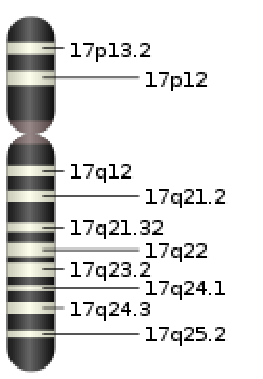
\includegraphics[height=5.7 cm]{figures/nchr17}
% \end{figure}
% \end{columns}
% \end{frame}

%%%%%%%%%%%%%%%%%%%%%%%%%%%%%%%%%%%%%%%%%%%%%%%%%%%%%%%%%%%%%%%%%%%%%%%%%%%%%%%%%%%%%%%%%%%%%

%%%%%%%%%%%%%%%%%%%%%%%%%%%%%%%%%%%%%%%%%%%%%%%%%%%%%%%%%%%%%%%%%%%%%%%%%%%%%%%%%%%%%%%%%%%%%%%%%%5555555%%%%%%%%%55

\begin{frame} {Story of a Statistician} 

\begin{figure}
\centering
  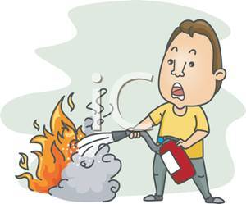
\includegraphics[width=0.8\textwidth]{figures/fire}
\end{figure}

\end{frame}

%%%%%%%%%%%%%%%%%%%%%%%%%%%%%%%%%%%%%%%%%%%%%%%%%%%%%%%%%%%%%%%%%%%%%%%%%%%%%%%%%%%%%%%%%%%%%%%%%%5555555%%%%%%%%%55

\begin{frame} {Importance of Using More Samples} 

\begin{itemize}\setlength{\itemsep}{7mm}
\item We expect that a sample of size 10 to be more informative than a sample of size 1 \\
\item A sample size of 100  more informative than 10, etc. \\ 
\item {\color{red} How much better?} \\
\item The answer is \textbf{The Square Root Law}
\end{itemize}

\vspace{2mm}
 
 $\text{Accuracy of information} = \sqrt \text{volume of information}$

 
% \begin{fquote}[{T. Mayer}] 
% Because these values were  derived from nine times as many observations one can therefore conclude that they are \st{nine} {\color {red} $\sqrt{9} = 3$ } times more correct.  
% \fqsource{{1750}} \end{fquote} 

\end{frame}

%%%%%%%%%%%%%%%%%%%%%%%%%%%%%%%%%%%%%%%%%%%%%%%%%%%%%%%%%%%%%%%%%%%%%%%%%%%%%%%%%%%%%%%%%%%%%%%%%%5555555%%%%%%%%%

\begin{frame} {The Multiresolution Data in Biology} 

\vspace{1mm}

\begin{figure}
\centering
  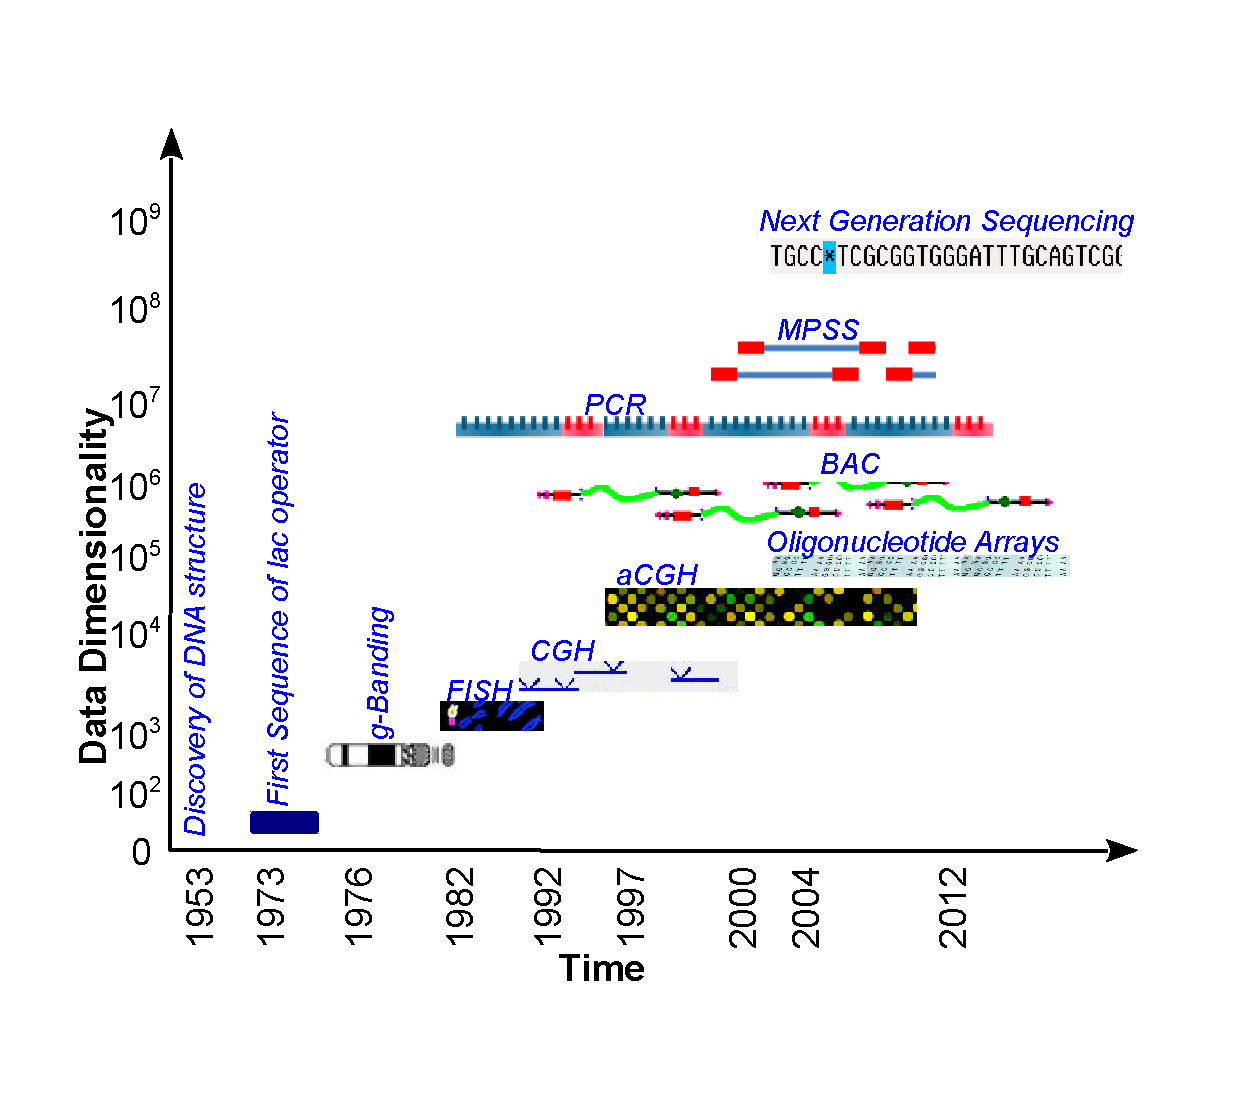
\includegraphics[trim=1cm 2cm 0.5cm 2.2cm, clip=true, width=0.75\textwidth]{figures/arraytypes}
\end{figure}

\vspace{-3mm}

\footnotesize
$\blacksquare$ Multiresolution data is everywhere: biology, computer vision, telecoms ...

$\blacksquare$ Older Generation Technology $\Rightarrow$ Data in Coarse Resolution

$\blacksquare$ Newer Generation Technology $\Rightarrow$ Data in Fine Resolution

%$\blacksquare$ \textbf{{\color{red}How to analyze data in multiple resolutions in a single analysis?}}

\end{frame}
%%%%%%%%%%%%%%%%%%%%%%%%%%%%%%%%%%%%%%%%%%%%%%%%%%%%%%%%%%%%%%%%%%%%%%%%%%%%%%%%%%%%%%%%%%%%%%%%%%%%%%%%%%%%%%%%%%


\begin{frame} {The Multiresolution Data in Biology} 

\vspace{1mm}

\begin{figure}
\centering
  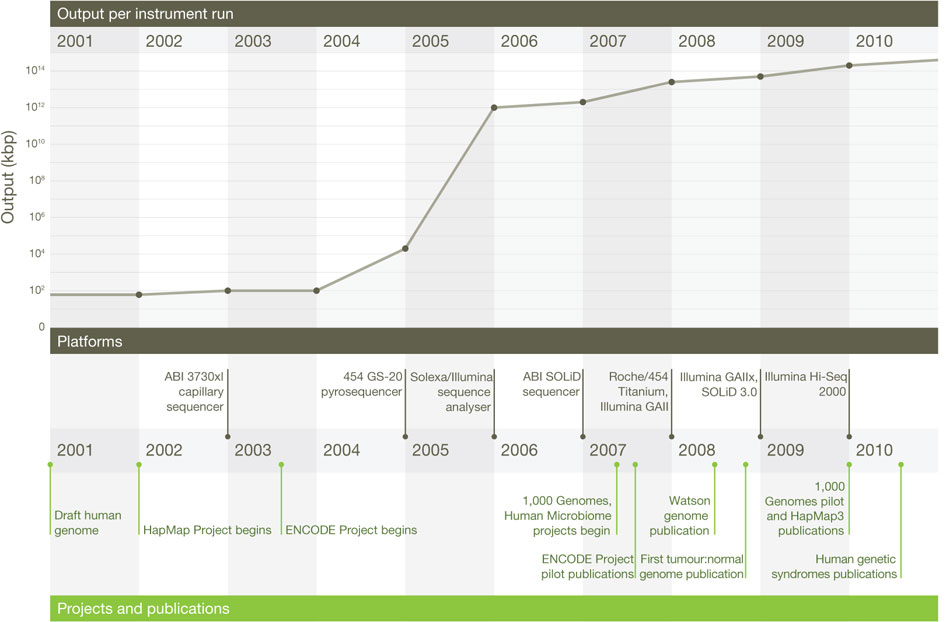
\includegraphics[trim=0cm 1cm 0.5cm 0.5cm, clip=true, width=0.98\textwidth]{figures/sequencing}
\end{figure}

\vspace{-3mm}

\footnotesize E. R. Mardis, \texttt{A decade's perspective on DNA sequencing technology}, \textbf{Nature}, 2011

\end{frame}

% \begin{frame} {Mixture Modelling of 0--1 Data} 
% \begin{itemize}\setlength{\itemsep}{2.5mm}
% %    \item Cancer is a collection of heterogeneous diseases  
% %    \item Data is 0--1 data: presence or absence of chromosomal aberrations
%     \item Finite Mixture Modelling of the Multivariate Bernoulli Distribution \\  
%     \vspace{0.1cm}  
% \textcolor{blue} { $ P(x) = \sum _{j=1}^{J} \pi _{j} P(x|\theta _{j}) = \sum _{j=1}^{J} \pi _{j} \prod _{i=1}^{d} \theta_{ji}^{x_i}(1-\theta _{ji})^{1-x_{i}}$ } \\
%       \vspace{0.1cm}
%      \item EM algorithm trains the Mixture Models using open-source BernoulliMix program package 
%      \href{http://users.ics.aalto.fi/jhollmen/BernoulliMix/}({ Available From Authors}) 
%      \item EM algorithm needs a priori knowledge of no. of components, $J$
%      \item Model selection based cross-validation with respect to likelihood determines the optimal $J$
% \end{itemize}
% \end{frame}

%%%%%%%%%%%%%%%%%%%%%%%%%%%%%%%%%%%%%%%%%%%%%%%%%%%%%%%%%%%%%%%%%%%%%%%%%%%%%%%%%%%%%%%%%%%%%%%%%%%%%%%%%%%%%%%%%%


% \begin{frame}{Chromosomal Aberrations Patterns in Cancer}
% \begin{itemize} \setlength{\itemsep}{6mm}
%   \item Abnormality in the normal chromosomal content of a cell
%   \item Different cases of DNA copy number aberrations
%   \begin{itemize}\setlength{\itemsep}{2.5mm}
%     \item Deletion: When the copy number $\boldsymbol{\textless 2} $ 
%     \item Duplication: When the copy number $\boldsymbol{\textgreater 2}$
%     \item Amplification: When the copy number $\boldsymbol {\gg 5}$
%   \end{itemize}
%   \item Why detect copy number aberrations?
%   \item DNA copy number aberrations are hallmarks of cancer
% \end{itemize}
% \end{frame}

%%%%%%%%%%%%%%%%%%%%%%%%%%%%%%%%%%%%%%%%%%%%%%%%%%%%%%%%%%%%%%%%%%%%%%%%%%%%%%%%%%%%%%%%%%%%%

\begin{frame}{DNA Copy Number Amplification Dataset}
\begin{figure}[h!]
  \centering
  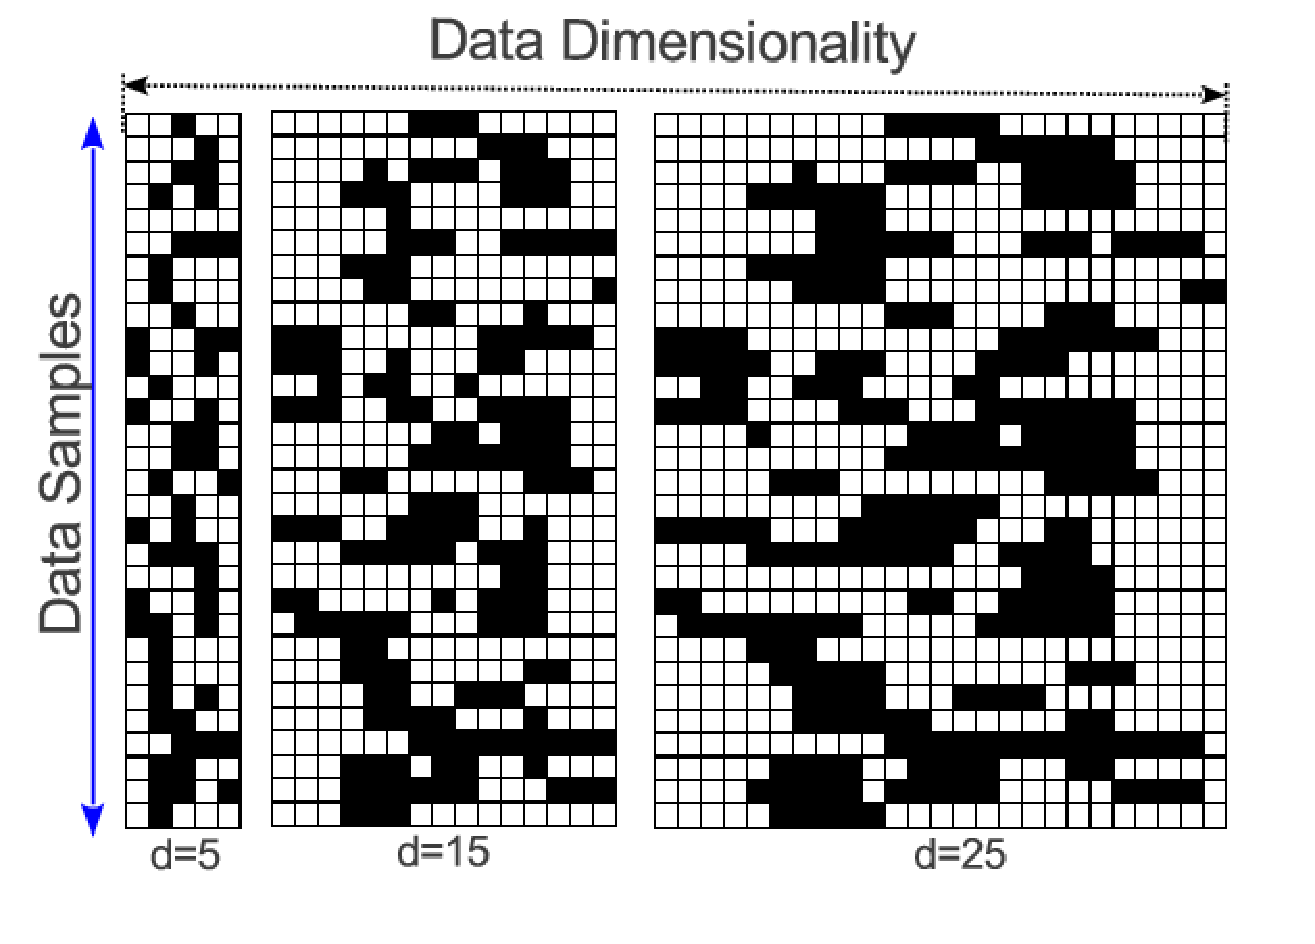
\includegraphics[height=0.8\textheight]{figures/datavis}
   \label{Fig:converge}
\end{figure}

\vspace{-6.5mm}

\textbf{{\color{red}How to analyze data in multiple resolutions in a single analysis?}}
\end {frame}

%%%%%%%%%%%%%%%%%%%%%%%%%%%%%%%%%%%%%%%%%%%%%%%%%%%%%%%%%%%%%%%%%%%%%%%%%%%%%%%%%%%%%%%%%%%%%

\begin{frame} {Mixture Modeling of Multiresolution 0--1 Data} 
\small
\begin{itemize}\setlength{\itemsep}{1mm}
    \item {\color{red} {Why Mixture Models?}}
    \item Cancer is a heterogeneous collection of several diseases and mixture models are well known for their ability to model heterogeneity
    \item Mixture models generally cannot model multiresolution data
    
    \vspace{-2mm}
    
      \begin{figure}
      \centering
      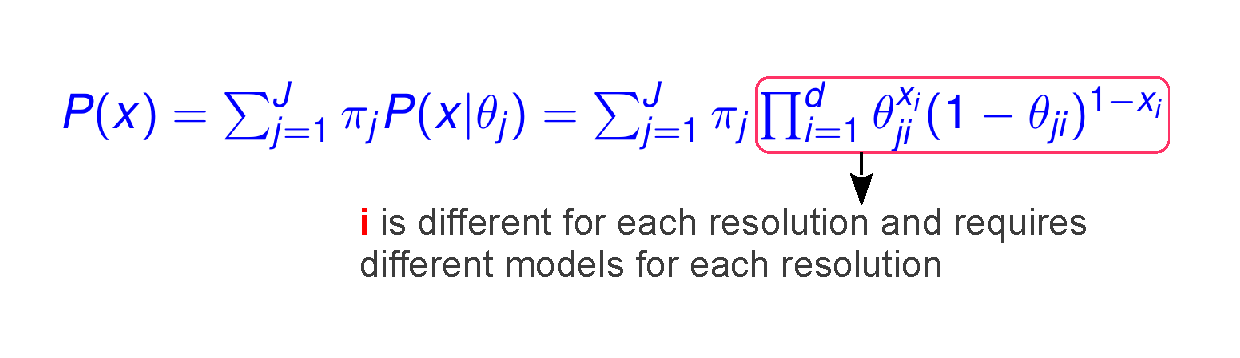
\includegraphics[trim=1cm 1.3cm 1cm 1.3cm, clip=true, width=0.9\textwidth]{figures/multieq}
      \end{figure}
      
          \vspace{-2mm}
   
     \item Multiresolution data can be transformed to single resolution for mixture modeling (Adhikari \& Hollm\'en, 2010 )
     \item Transformation in the model domain initiates interactions between the models (Adhikari \& Hollm\'en, 2012 )
     \item Bayesian Networks as Mixture Components in the mixture model (Adhikari \& Hollm\'en, 2013)
\end{itemize}
\end{frame}

%%%%%%%%%%%%%%%%%%%%%%%%%%%%%%%%%%%%%%%%%%%%%%%%%%%%%%%%%%%%%%%%%%%%%%%%%%%%%%%%%%%%%%%%%%%%%%%%%%%%%%%%%%%%%%%%%%

\begin{frame} {Mixture Models of Chromosomal Aberrations Data} 

      \begin{figure}
      \centering
      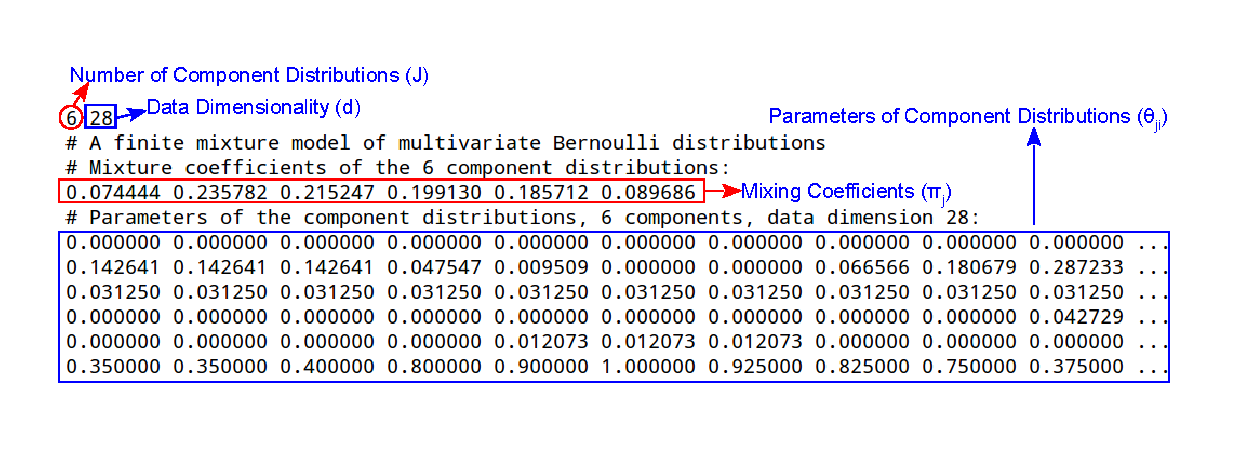
\includegraphics[trim=1cm 1cm 1cm 1cm, clip=true, width=0.99\textwidth]{figures/mixmdl11}
      \end{figure}
      
Only 10 of 28 dimensions of Chromosome 1 is shown.
\pause 
 \begin{fquote}[{John Tukey}] 
An approximate answer to the right problem is worth a good deal more than an exact answer to an approximate problem.
 \fqsource{{Super Freakonomics}} \end{fquote} 

%"An approximate answer to the right problem is worth a good deal more than an exact answer to an approximate problem." -- John Tukey

%"Data do not speak for themselves - they need context, and they need skeptical evaluation" Allen Wilcox


\end{frame}

%%%%%%%%%%%%%%%%%%%%%%%%%%%%%%%%%%%%%%%%%%%%%%%%%%%%%%%%%%%%%%%%%%%%%%%%%%%%%%%%%%%%%%%%%%%%%%%%%%%%%%%%%%%%%%%%%%


\begin{frame} {Structural Visualization of 0-1 Data} 

      \begin{figure}
      \centering
      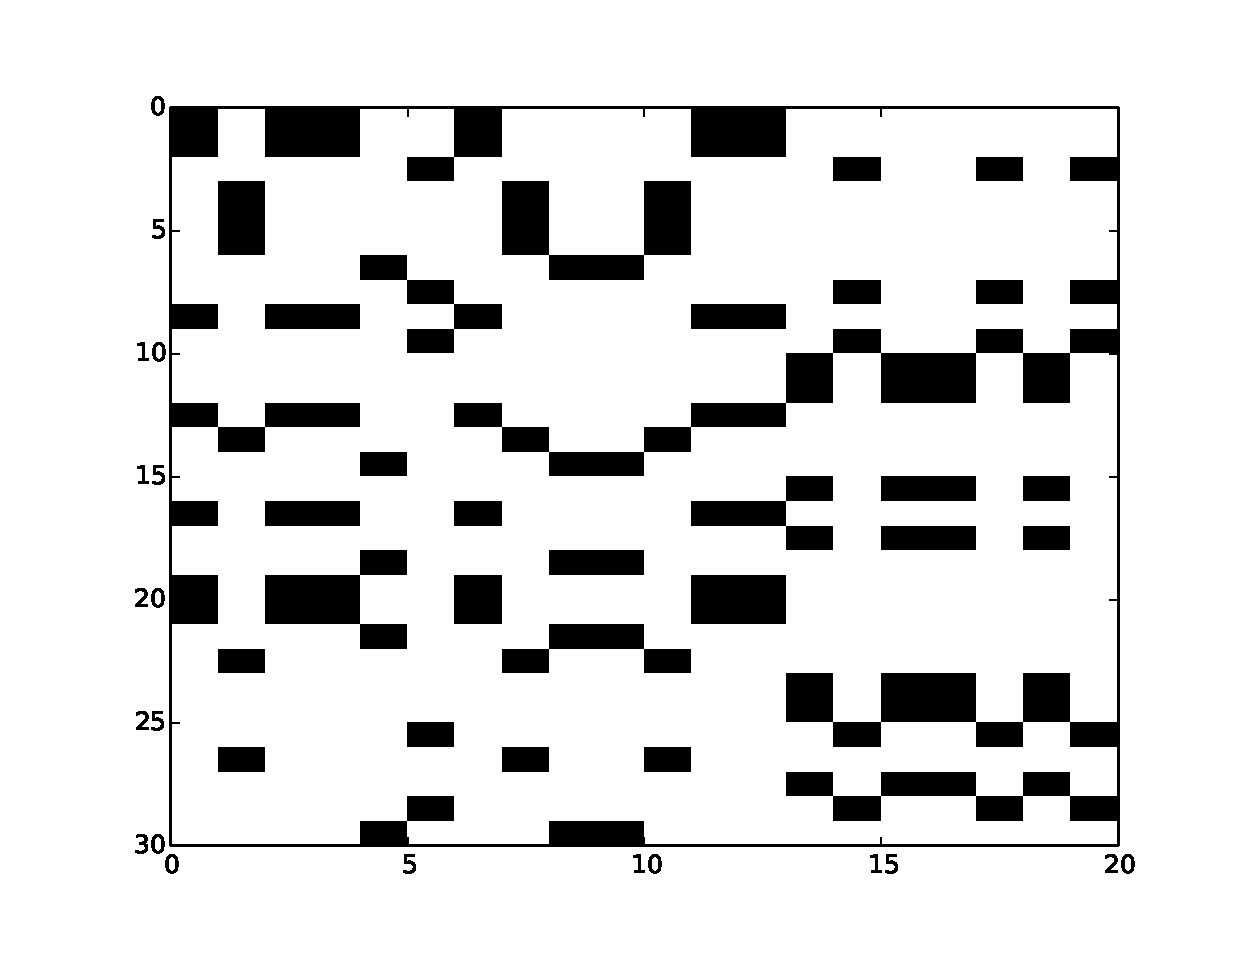
\includegraphics[trim=1cm 0.5cm 1cm 1cm, clip=true, width=0.7\textwidth]{figures/scrambled}
      \end{figure}
      
      \begin{itemize}\setlength{\itemsep}{1mm}
      \item What if I told you there is no structure in the data? 
      \pause \item \textcolor {red}{What if I told you there are \textbf{7} clusters in the data?} 
      \end{itemize}
       
     
\end{frame}

%%%%%%%%%%%%%%%%%%%%%%%%%%%%%%%%%%%%%%%%%%%%%%%%%%%%%%%%%%%%%%%%%%%%%%%%%%%%%%%%%%%%%%%%%%%%%%%%%%%%%%%%%%%%%%%%%%


\begin{frame} {Structural Visualization of Clusters in the Data} 

      \begin{figure}
      \centering
      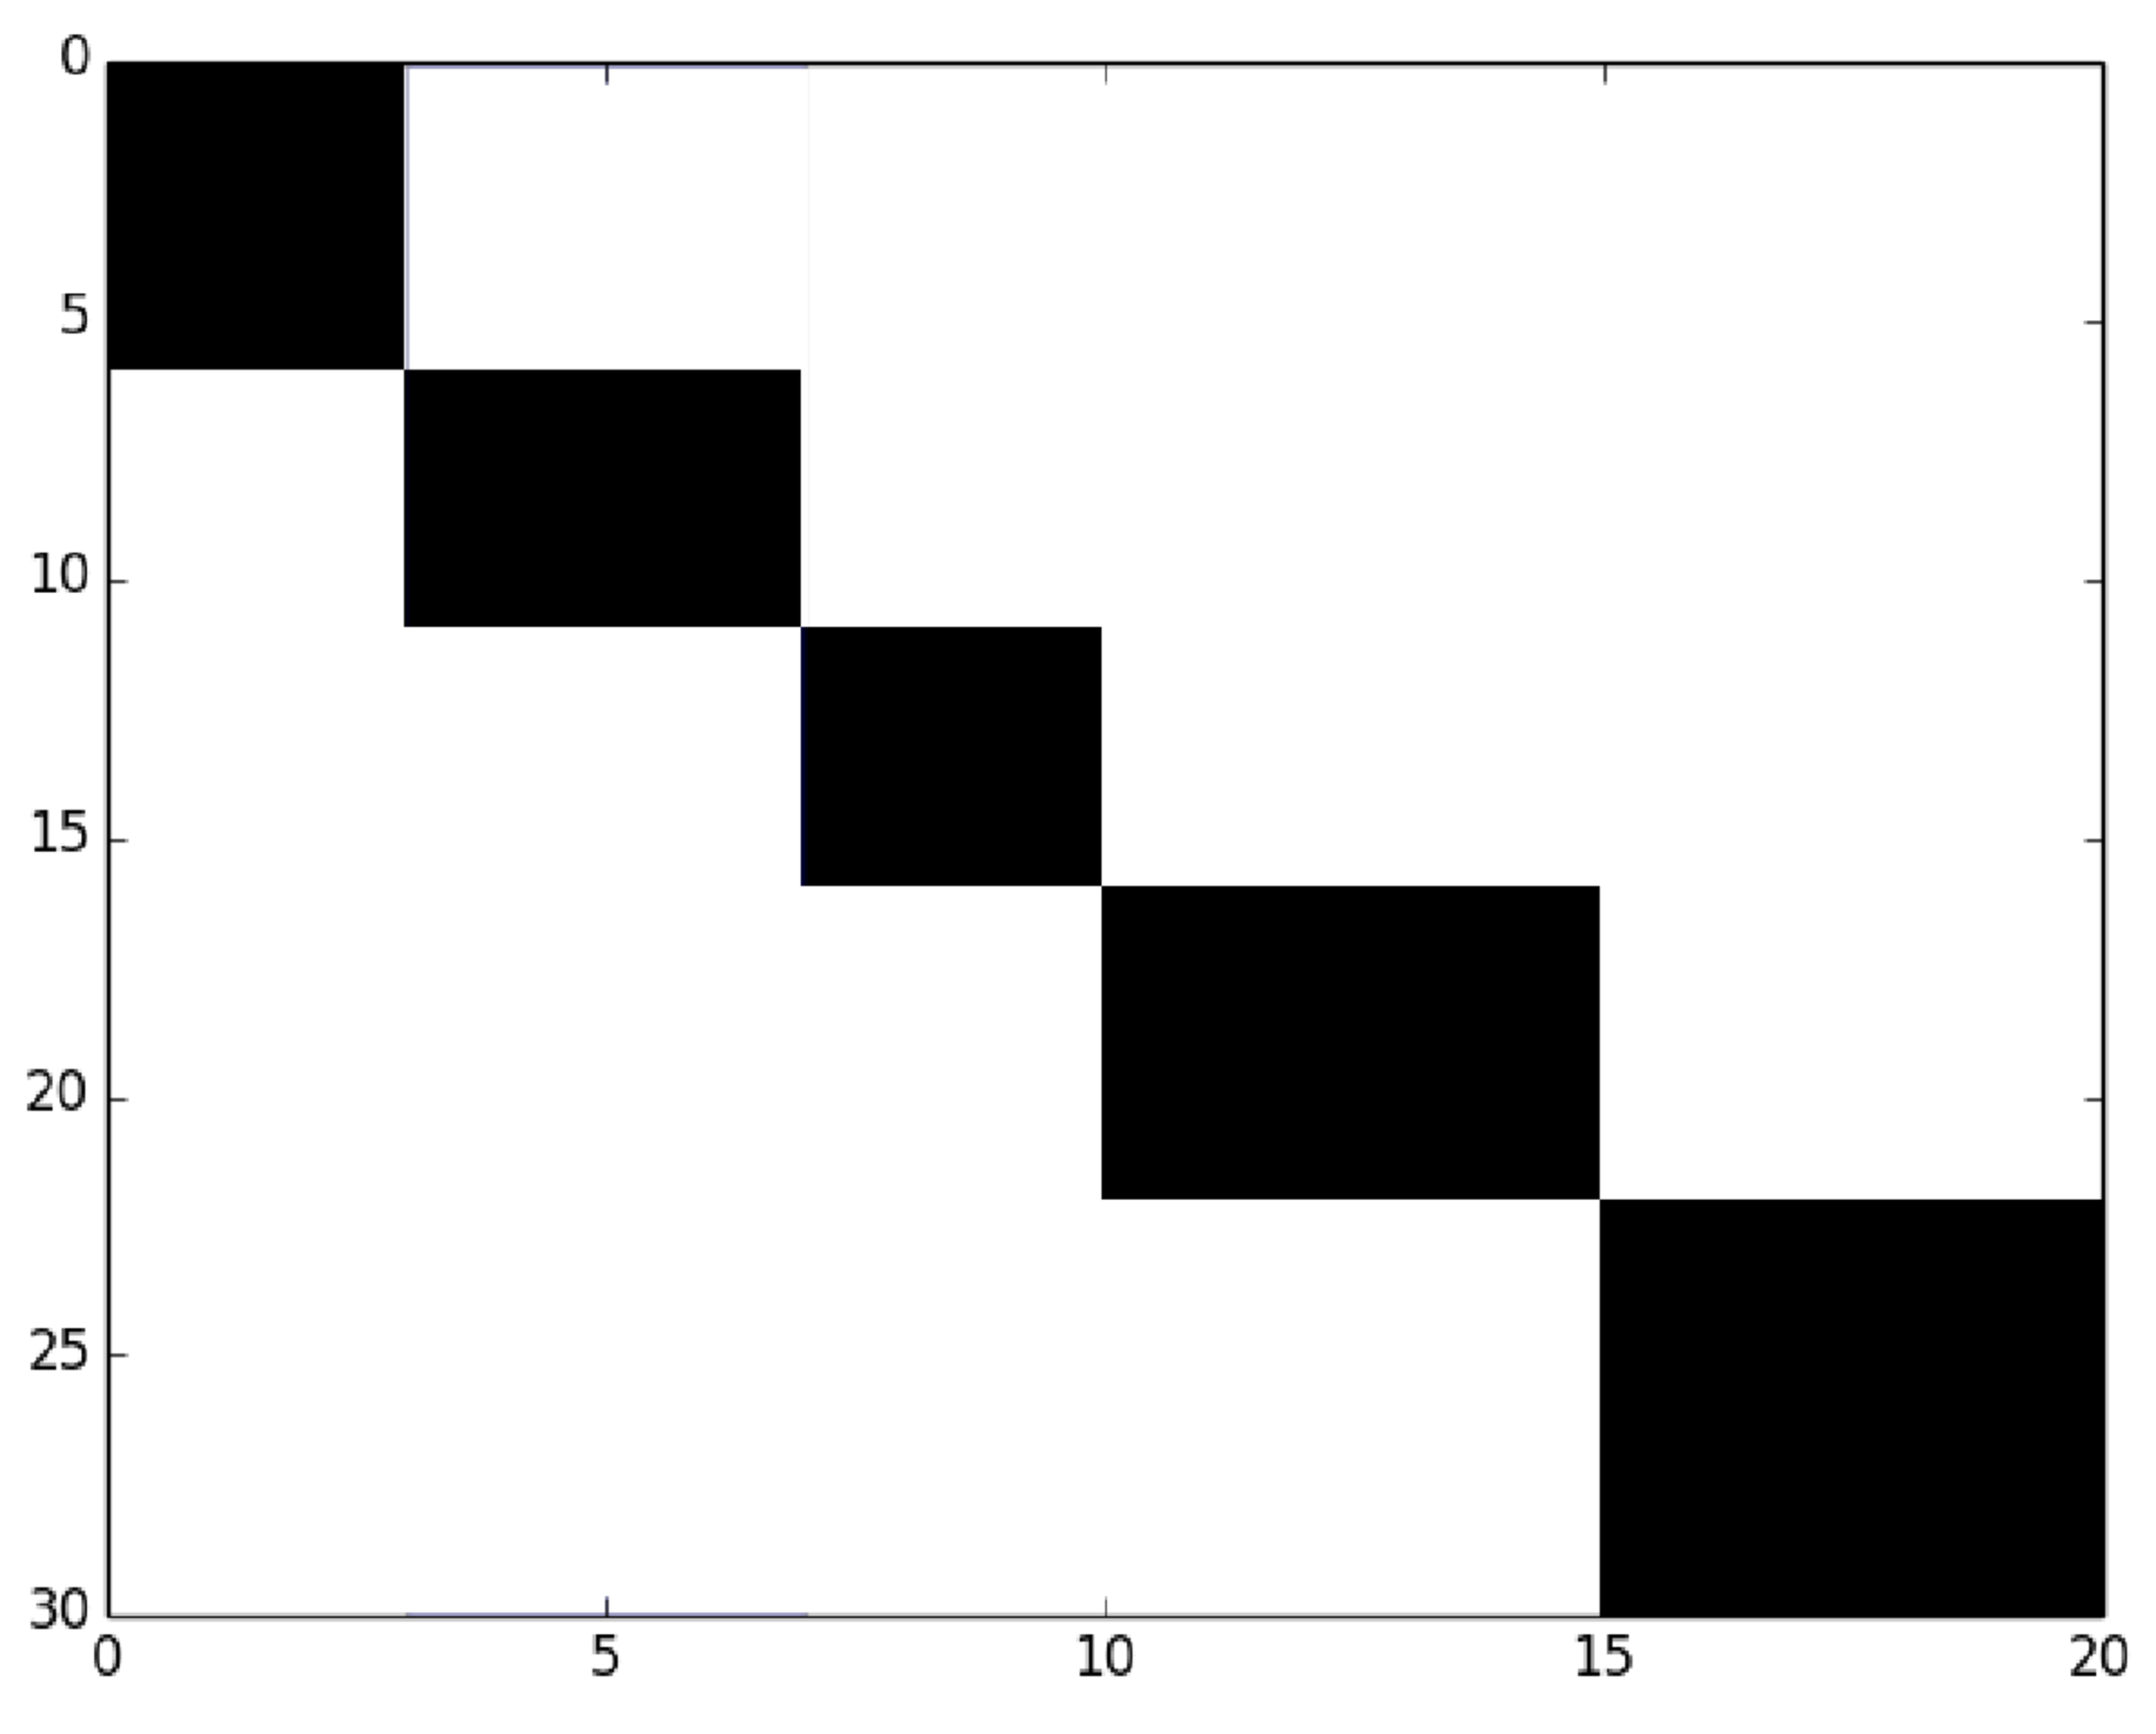
\includegraphics[trim=0cm 0cm 0cm 0cm, clip=true, width=0.55\textwidth]{figures/banded}
      \end{figure}
      
      \begin{itemize}\setlength{\itemsep}{1mm}
      
\small
\item Using banded matrices, we can expose the banded structure 
\item We can overlay cluster information over banded structure 
\pause \item \textcolor {red} { But what if we can not shuffle columns of genome?}
\end{itemize}

\end{frame}

%%%%%%%%%%%%%%%%%%%%%%%%%%%%%%%%%%%%%%%%%%%%%%%%%%%%%%%%%%%%%%%%%%%%%%%%%%%%%%%%%%%%%%%%%%%%%%%%%%%%%%%%%%%%%%%%%%

\begin{frame} {Clusters overlayed on banded structure of data} 

      \begin{figure}
      \centering
      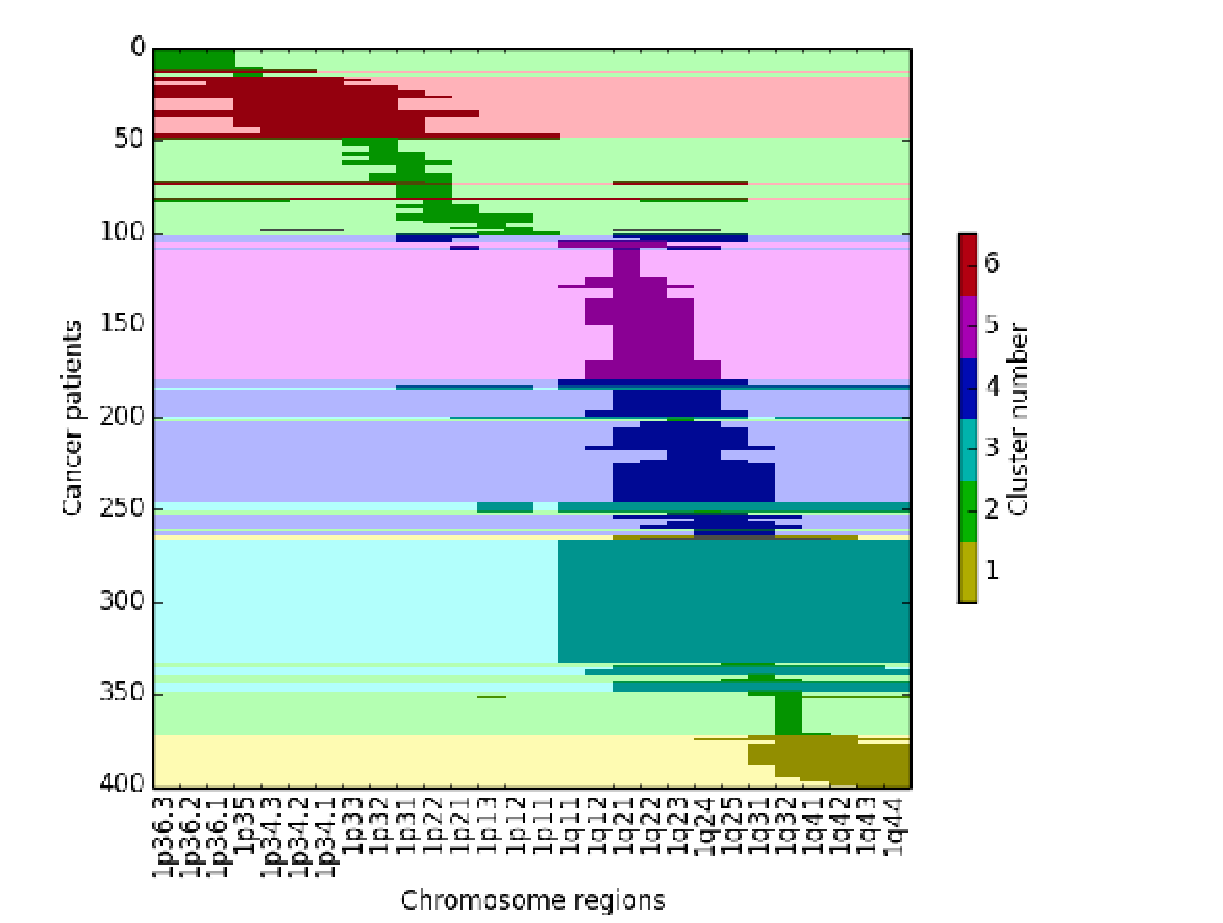
\includegraphics[trim=1cm 0cm 1cm 1cm, clip=true, width=0.8\textwidth]{figures/cluscolors}
      \end{figure}
      
      \vspace{-5mm}
      

\end{frame}



%%%%%%%%%%%%%%%%%%%%%%%%%%%%%%%%%%%%%%%%%%%%%%%%%%%%%%%%%%%%%%%%%%%%%%%%%%%%%%%%%%%%%%%%%%%%%%%%%%%%%%%%%%%%%%%%%%

\begin{frame} {Semantic Data Mining} 

\begin{fquote}[{ Allen Wilcox}] 
Data do not speak for themselves -- they need context, and they need skeptical evaluation  
\fqsource{{Harvard Professor}} \end{fquote}

% \begin{fquote}[{ Prem}] 
%  Data is by nature social   
% \fqsource{{}} \end{fquote}
% 
% \vspace{-5mm}

\begin{itemize}\setlength{\itemsep}{1mm}
\small
\item Abundance of ontologies and semantically annotated data collections (Semantic Web)
\item Biological systems are complex consisting of interwoven subsystems 
\item Increasing volume of Semistructured, heterogeneous and distributed data
\end{itemize}
      

\end{frame}

%%%%%%%%%%%%%%%%%%%%%%%%%%%%%%%%%%%%%%%%%%%%%%%%%%%%%%%%%%%%%%%%%%%%%%%%%%%%%%%%%%%%%%%%%%%%%%%%%%%%%%%%%%%%%%%%%%

%\begin{frame} {Semantic Data Mining} 
%
%% \begin{fquote}[{ \sout{Aristotle} Prem}] 
%% \sout{Man} Data is by nature \sout{a} social \sout{animal}.  
%% \fqsource{{ \sout{Greek philosopher} Doctoral Student}} \end{fquote}
%
%
%Similarly, data also can not stand alone, esp. in Biology.
%
%\begin{itemize}\setlength{\itemsep}{1mm}
%      
%\small
%\item Abundance of ontologies and semantically anotated data collections (Semantic Web)
%\item Biological systems are complex consisting of interwoven subsystems 
%\item Increasing volume of Semi-??structured, heterogeneous and distributed data, 
%\item Semantic data mining algorithms addresses the challenge of mining abundance of knowledge encoded in domain ontologies
%constrained by the heuristics computed from the empirical data
%
%\end{itemize}
%      
%
%\end{frame}


%%%%%%%%%%%%%%%%%%%%%%%%%%%%%%%%%%%%%%%%%%%%%%%%%%%%%%%%%%%%%%%%%%%%%%%%%%%%%%%%%%%%%%%%%%%%%%%%%%%%%%%%%%%%%%%%%%

\begin{frame} {Semantic Data Mining} 

      \begin{figure}
      \centering
      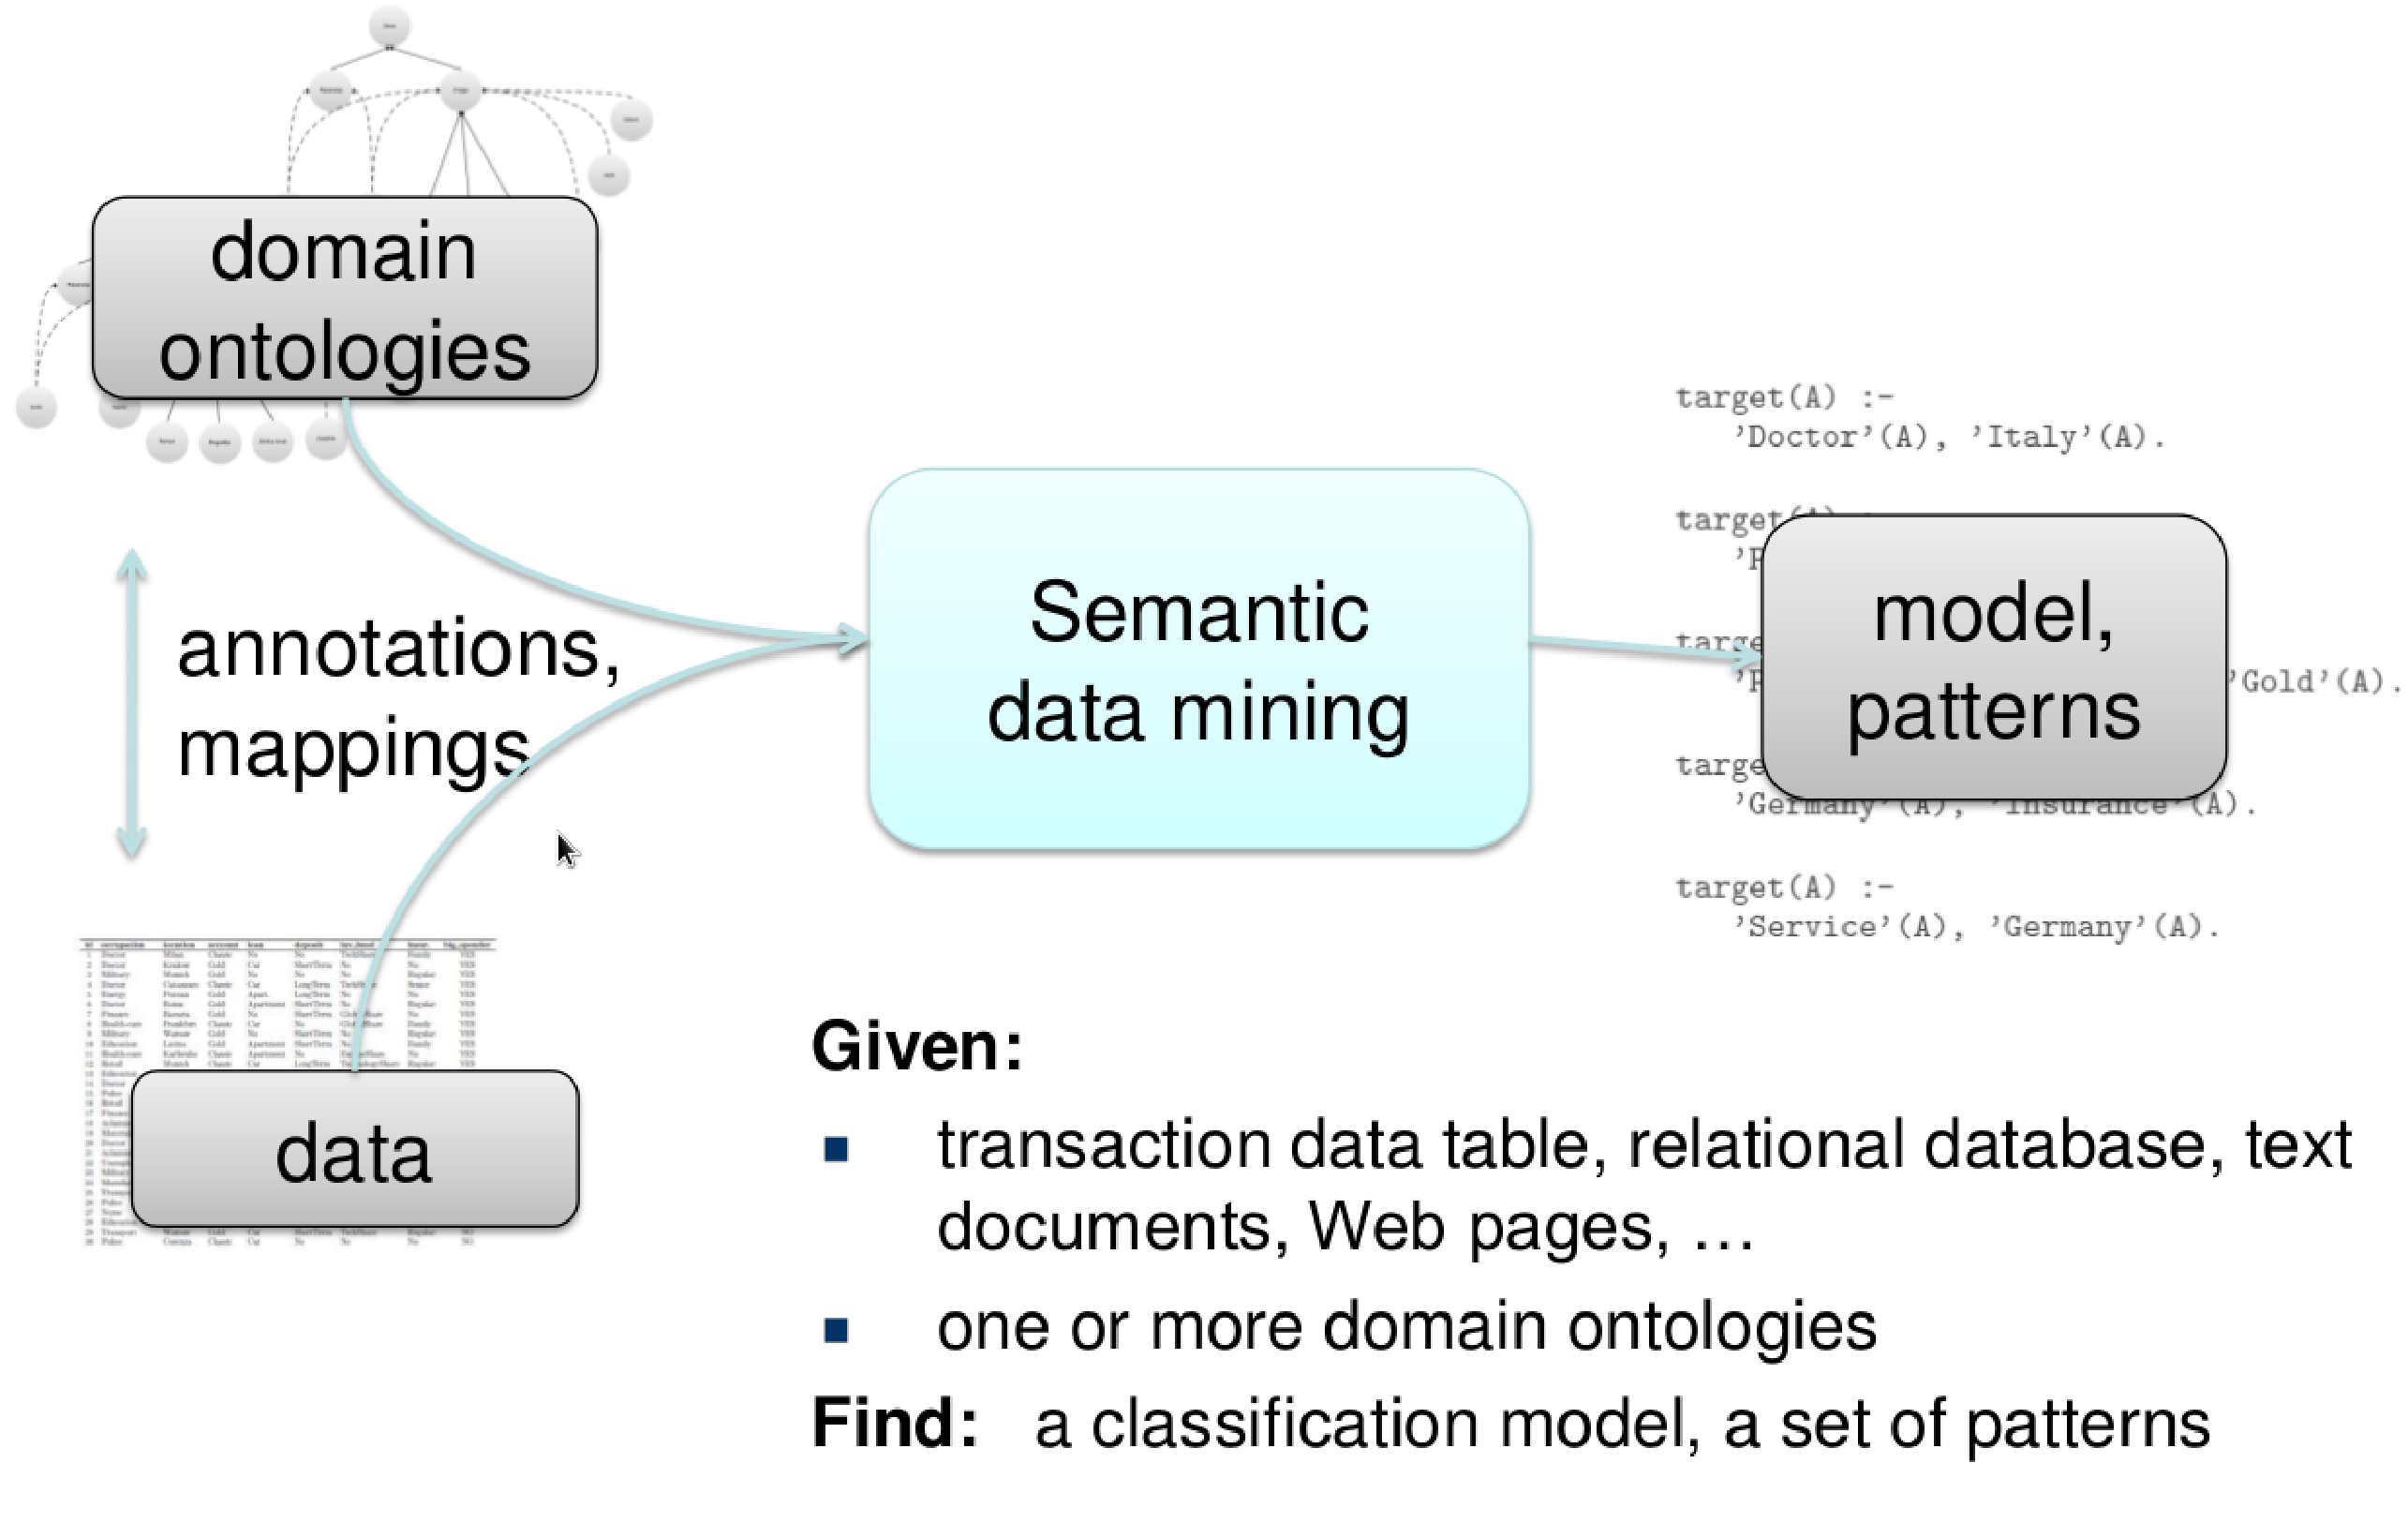
\includegraphics[trim=1cm 0.5cm 1cm 1cm, clip=true, width=0.9\textwidth]{figures/semantic}
      \end{figure}
      
      \vspace{-5mm}
Hedwig semantic pattern mining algorithm (A. Vavpeti\v{c}, V. Podpe\v{c}an, \& N. Lavra\v{c}, 2013)

\end{frame}

%%%%%%%%%%%%%%%%%%%%%%%%%%%%%%%%%%%%%%%%%%%%%%%%%%%%%%%%%%%%%%%%%%%%%%%%%%%%%%%%%%%%%%%%%%%%%%%%%%%%%%%%%%%%%%%%%%

\begin{frame} {Semantic Data Mining Rules for Cluster 3} 

      \begin{figure}
      \centering
      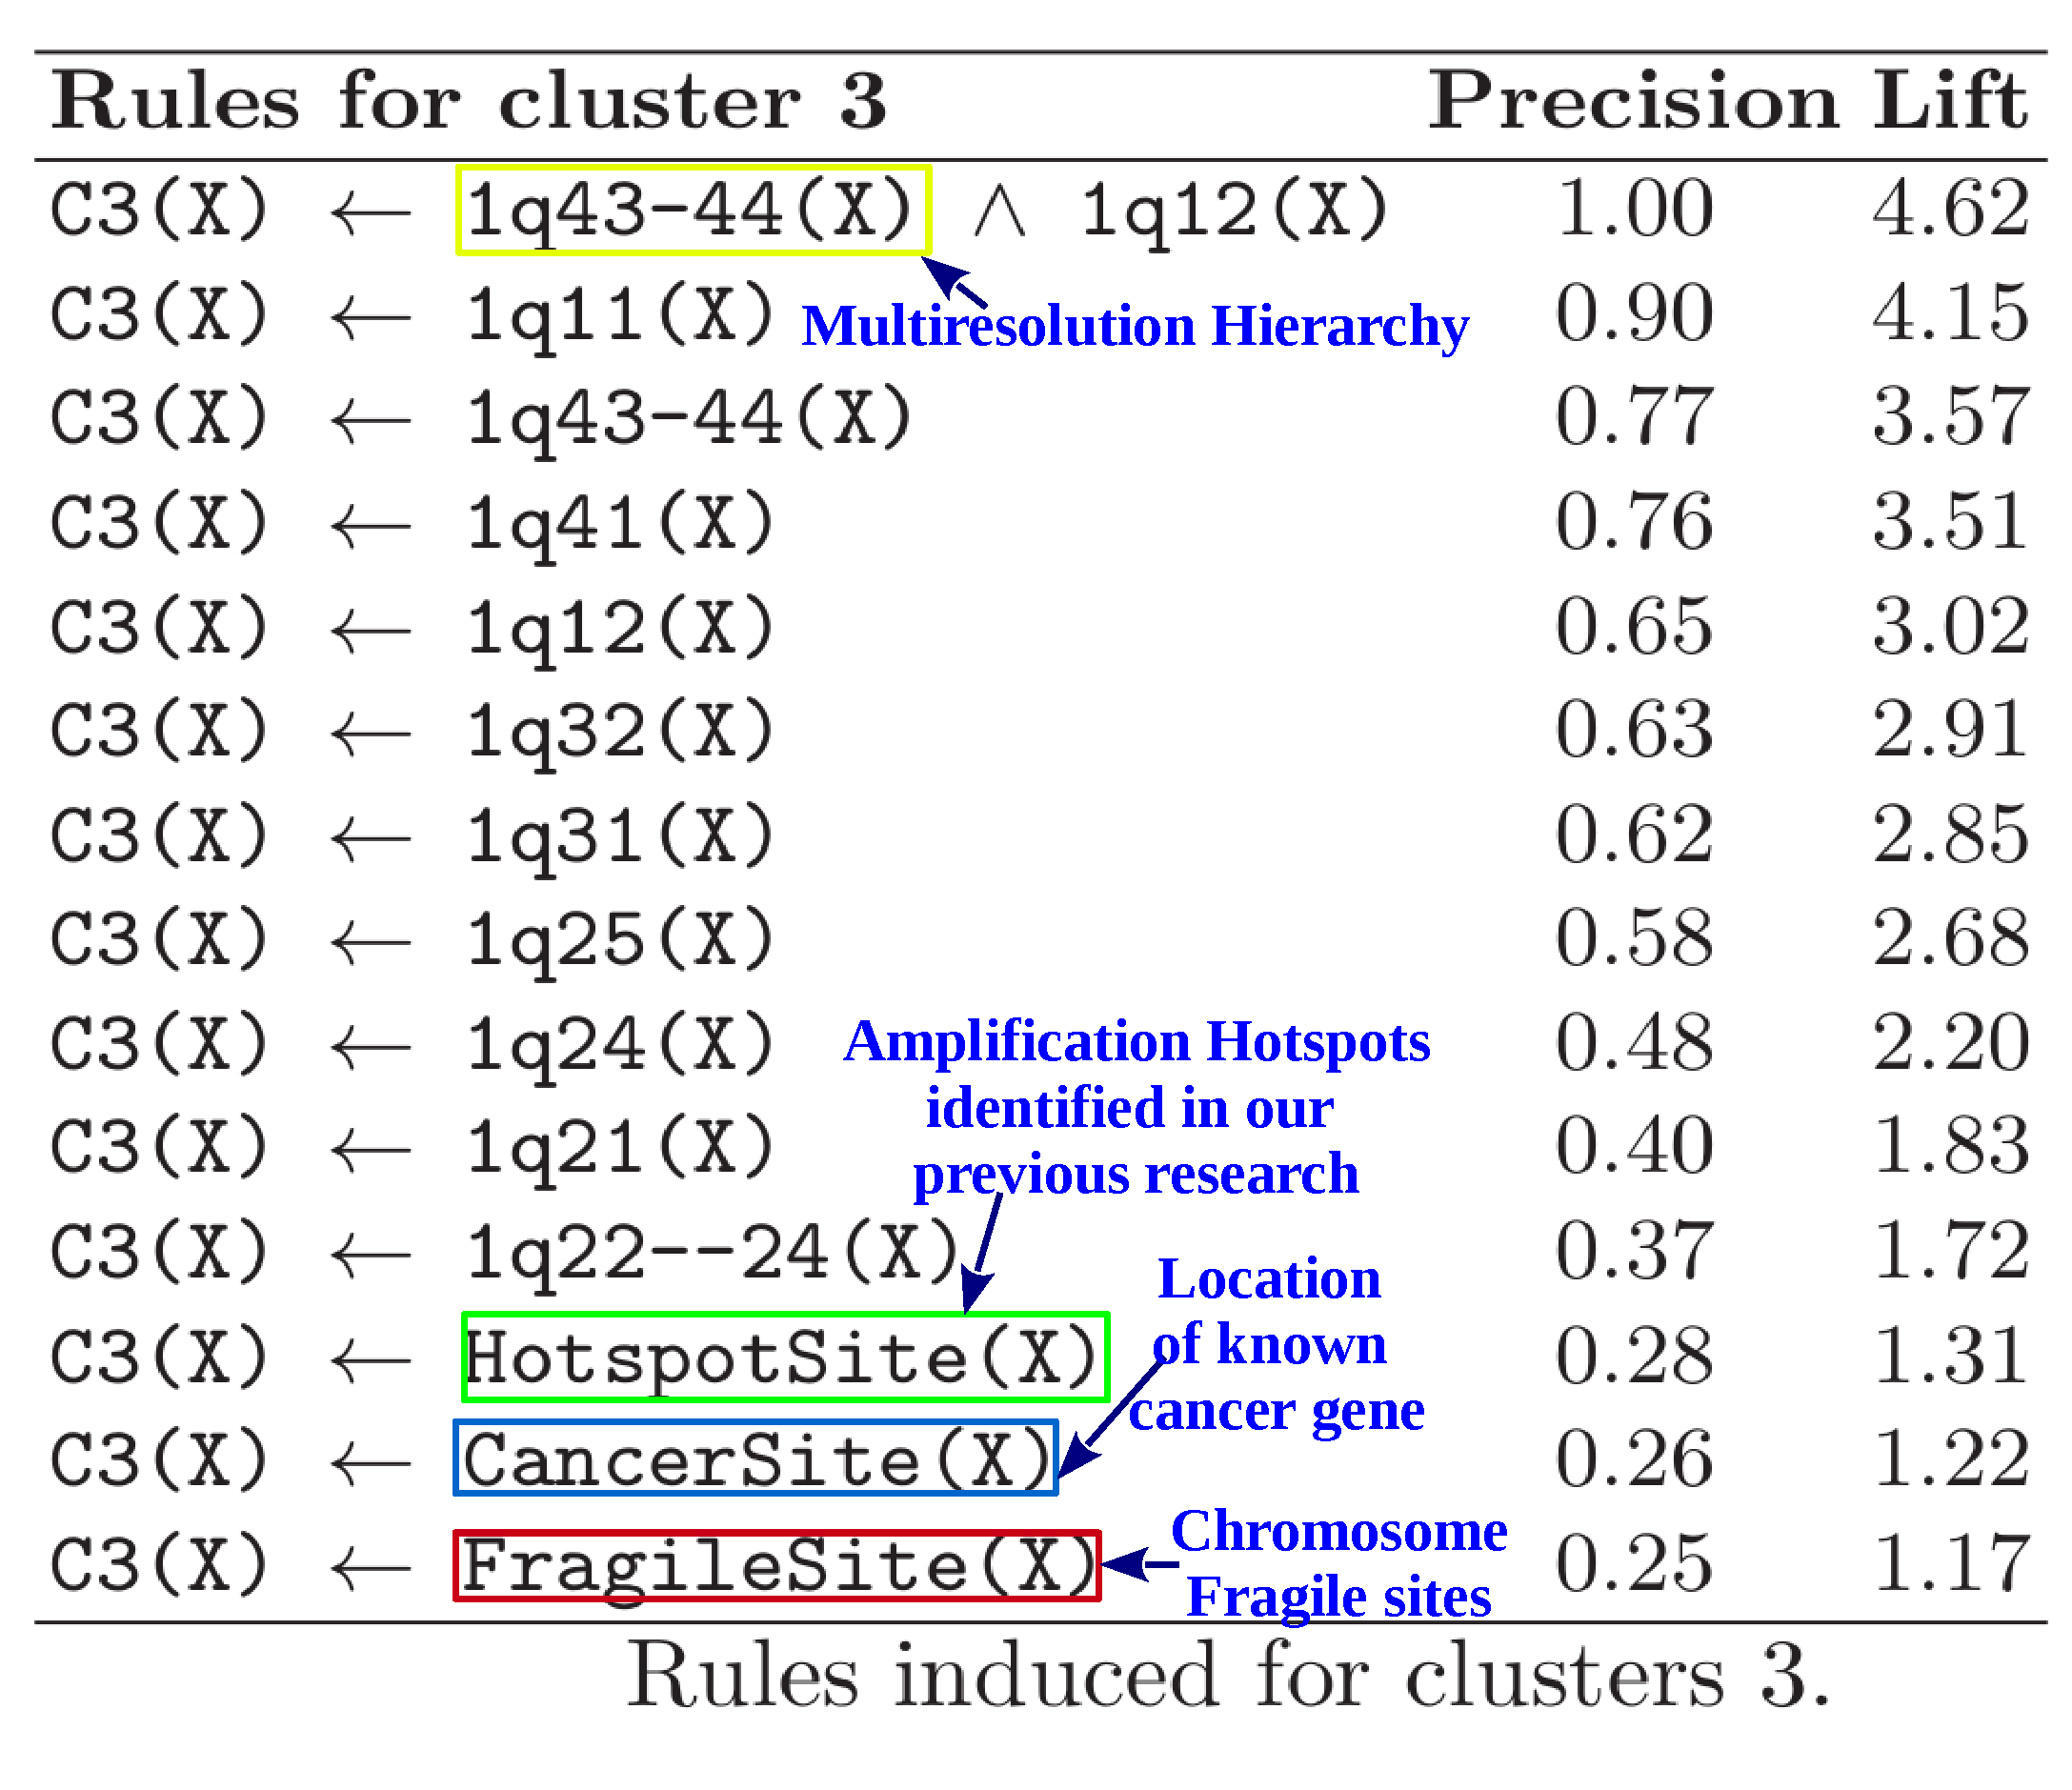
\includegraphics[trim=0cm 0cm 0cm 0cm, clip=true, width=0.8\textwidth]{figures/cluster3}
      \end{figure}
      
%       \vspace{-5mm}
%       
% \scriptsize Additional background knowledge used are: taxonomies of hierarchical structure of multiresolution amplification data, chromosomal locations
% of fragile sites, virus integration sites, cancer genes, and amplification hotspots

\end{frame}

%%%%%%%%%%%%%%%%%%%%%%%%%%%%%%%%%%%%%%%%%%%%%%%%%%%%%%%%%%%%%%%%%%%%%%%%%%%%%%%%%%%%%%%%%%%%%%%%%%%%%%%%%%%%%%%%%%

\begin{frame} {Semantic Data Mining Rules and Clusters} 

      \begin{figure}
      \centering
      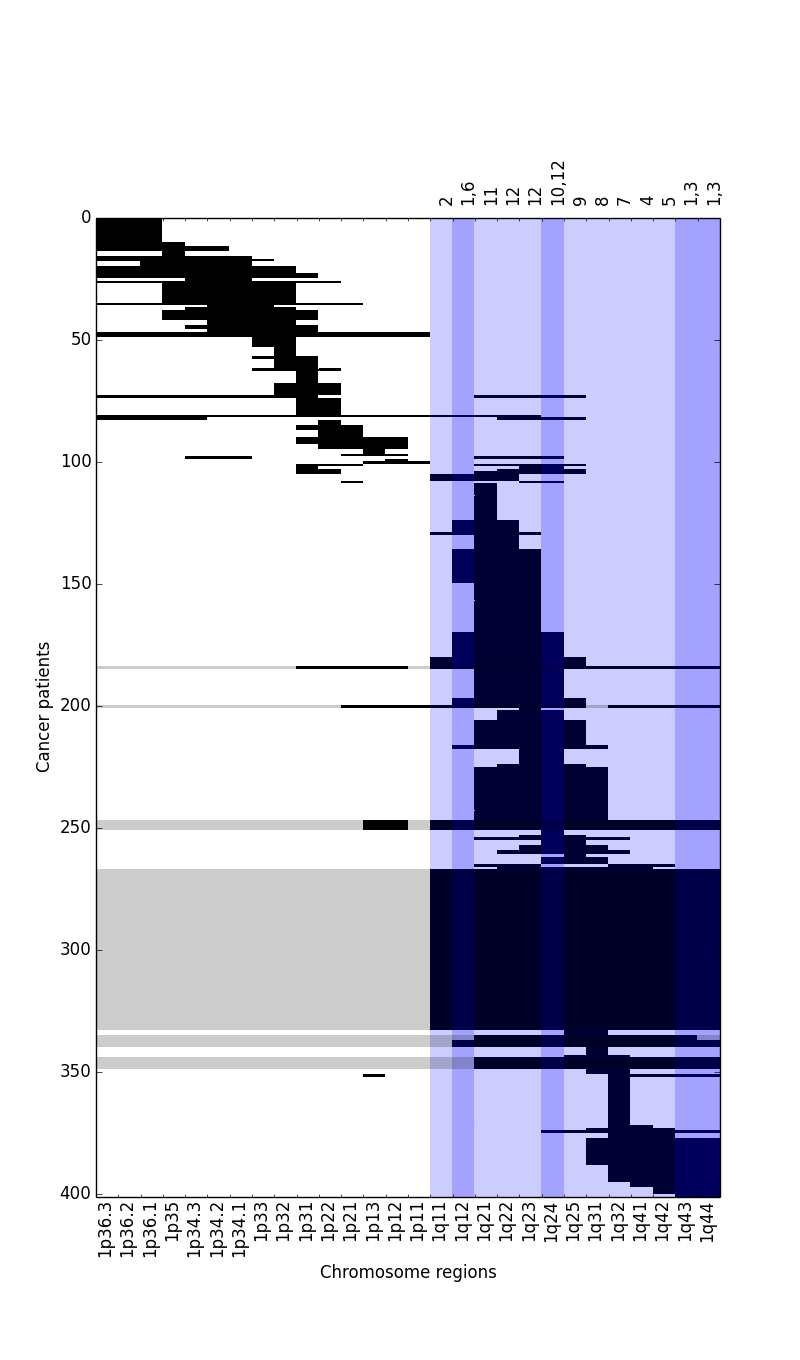
\includegraphics[trim=0cm 1.5cm 0cm 2cm, clip=true, width=0.45\textwidth]{figures/rules.png}
      \end{figure}
      
 %     \vspace{-5mm}      

\end{frame}

%%%%%%%%%%%%%%%%%%%%%%%%%%%%%%%%%%%%%%%%%%%%%%%%%%%%%%%%%%%%%%%%%%%%%%%%%%%%%%%%%%%%%%%%%%%%%%%%%%%%%%%%%%%%%%%%%%


\begin{frame}{Summary and Conclusions}

  \begin{figure}
      \centering
      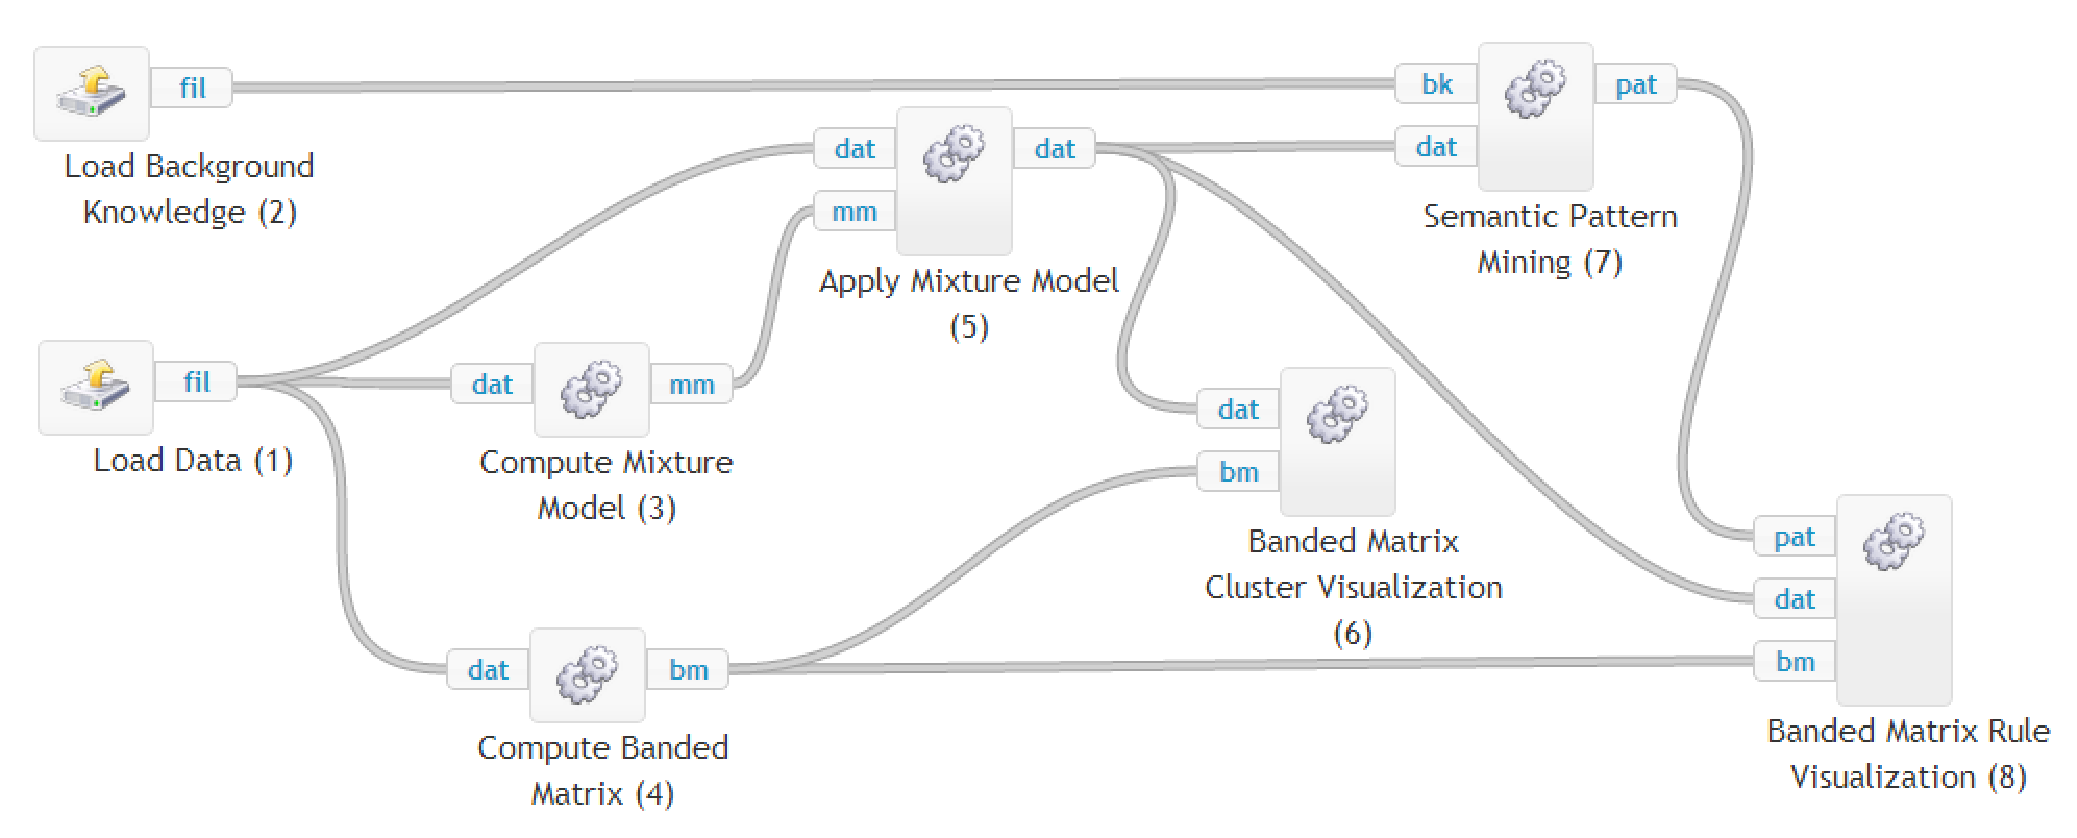
\includegraphics[trim=1cm 0cm 0cm 0cm, clip=true, width=0.99\textwidth]{figures/workflow}
      \end{figure}
      
 %     \vspace{-5mm}   
\end{frame}


%%%% QUESTIONS FRAME BELOW %%%%%%
%%%%%%%%%%%%%%%%%%%%%%%%%%%%%%%%%%%%%%%%%%%%%%%%%%%%%%%%%%%%%%%%%%%%%%%%%%%%%%%%%%%%%%%%%%%%%



\begin{frame}
 \frametitle{Questions, Comments, and Feedback}
 \begin{figure}[h!]
 \centering
 
\includegraphics[trim=1cm 1.5cm 1cm 3cm, clip=true, width=0.9\textwidth]{figures/questions}
 \end{figure}
 
%  \vspace{-15mm}
%  
%  \begin{figure}[h!]
%  \centering
%  
\includegraphics[width=0.8\textwidth]{figures/logoslong}
%  \end{figure}
 
%  \vspace{-5mm}
%  
%  \small The work is funded by Helsinki Doctoral Programme in Computer Science--Advanced Computing and Intelligent Systems (Hecse)
 \end{frame}
 
%%%%%%%%%%%%%%%%%%%%%%%%%%%%%%%%%%%%%%%%%%%%%%%%%%%%%%%%%%%%%%%%%%%%%%%%%%%%%%%%%%%%%%%%%%%%%
\end{document}
